\documentclass{beamer}

\usepackage{graphicx}
\usepackage{appendixnumberbeamer}

\title{DCT - Diszkrét koszinusz-transzformáció az adattömörítésben}
\author{Patka Zsolt-András}
\institute{Sapientia EMTE - Számítástechnika IV}
\date{2020.03.26}

\begin{document}

\begin{frame}
    \titlepage
\end{frame}

\begin{frame}
\frametitle{Miről lesz szó?}
\tableofcontents
\end{frame}

\section{Adattömörítés}

\subsection{Veszteségmentes adattömörítés}
\begin{frame}{\secname : \subsecname}
\begin{itemize}
    \item Lehetséges a tömörített adatból az eredeti adatok pontos rekonstrukciója
    \item Huffman
    \begin{itemize}
    \item változó hosszuságú kódok
    \item gyakrabban előfordult szimbólumok rövidebb kódot kapnak
    \item 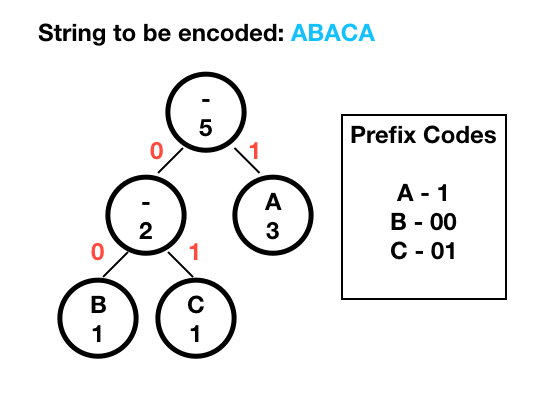
\includegraphics[scale=0.3]{figures/huffman.png} 
    \begin{footnotesize}
        forrás: \url{www.journaldev.com/23246/huffman-coding-algorithm}
        \end{footnotesize}
    \end{itemize}
    \item Például: Szöveges állományok tömörítése
\end{itemize}    
\end{frame}

\subsection{Veszteséges adattömörítés}
\begin{frame}{\secname : \subsecname}
\begin{itemize}
    \item A tömörített adatból az eredeti adatok nem pontos rekonstrukcióját teszi lehetővé
    \item Például: képek (JPEG), videók tömörítése (MPEG, H.26X)
\end{itemize}    
\end{frame}

\section{DCT}

\subsection{Fourier-transzformáció}
\begin{frame}{\secname : \subsecname}
    \begin{itemize}
        \item Periódikus jel felírása szinuszok és koszinuszok kombinációjaként
        \item $ X_k = \sum_{n=0}^{N - 1} x_n * [\cos(\frac{2 \pi}{N} kn) - i * sin(\frac{2\pi}{N} kn)]$
    \end{itemize}
\end{frame}

\subsection{DCT}
\begin{frame}{\secname : \subsecname}
    \begin{itemize}
        \item DCT-I:
        \begin{itemize}
            \item $ X_k = \frac{1}{2} (x_0 + (-1)^kx_{N-1}) + \sum_{n=0}^{N - 1} x_n * \cos[\frac{\pi}{N - 1} nk]$
        \end{itemize}
        \item DCT-II:
        \begin{itemize}
            \item $ X_k = \sum_{n=0}^{N - 1} x_n * \cos[\frac{\pi}{N} * (n + \frac{1}{2})k] $ $k=0,...,N-1$
            \item leggyakrabban használt forma (JPEG-ben is használt)
        \end{itemize}
    \end{itemize}
    
\end{frame}


\section{Alkalmazása - JPEG}

\subsection{Áttekintés}
\begin{frame}{\secname : \subsecname}
\centering
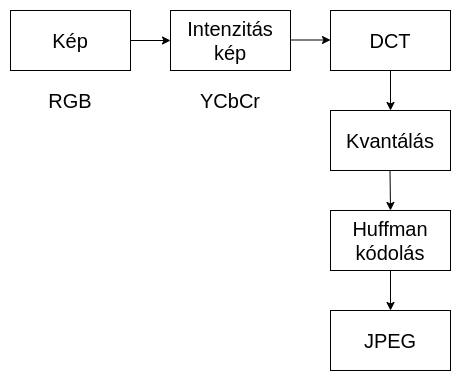
\includegraphics[scale=0.32]{figures/JPEG proc.png}

\begin{itemize}
    \item az emberi szem a világosságra sokkal érzékenyebb, mint a színre
    \item az emberi szem a magas frekvenciájú változásokat sokkal kevésébé érzékeli, mint az alacsony frekvenciájú változásokat
\end{itemize}

\end{frame}

\subsection{Downsampling}
\begin{frame}{\secname : \subsecname}

\begin{columns}
\begin{column}{0.3\textwidth}

RGB $\leftarrow$ YCbCr

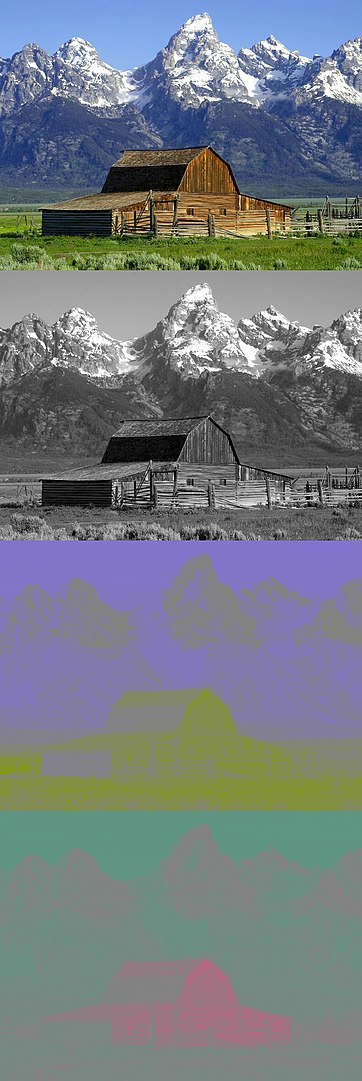
\includegraphics[scale=0.1]{figures/ycbcr.jpg}

\begin{footnotesize}
    forrás: \url{en.wikipedia.org/wiki/YCbCr}
\end{footnotesize}
\end{column}
\begin{column}{0.7\textwidth}

Downsampling:

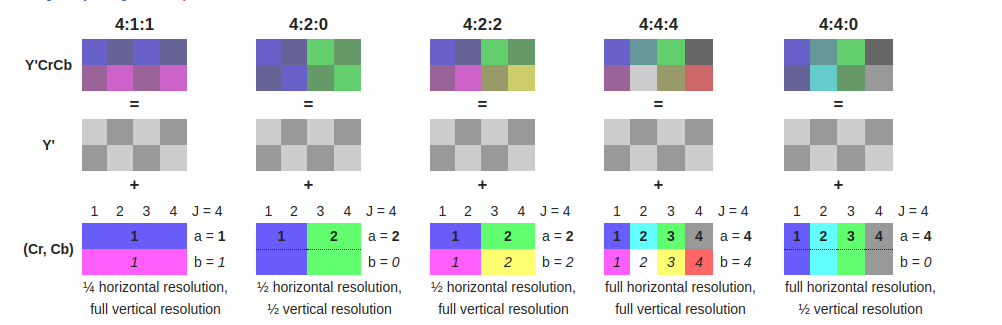
\includegraphics[scale=0.3]{figures/Downsampling.png}

\begin{footnotesize}
    forrás: \url{en.wikipedia.org/wiki/Chroma\_subsampling}
\end{footnotesize}

\end{column}
\end{columns}

\end{frame}

\subsection{DCT}
\begin{frame}{\secname : \subsecname}
\centering
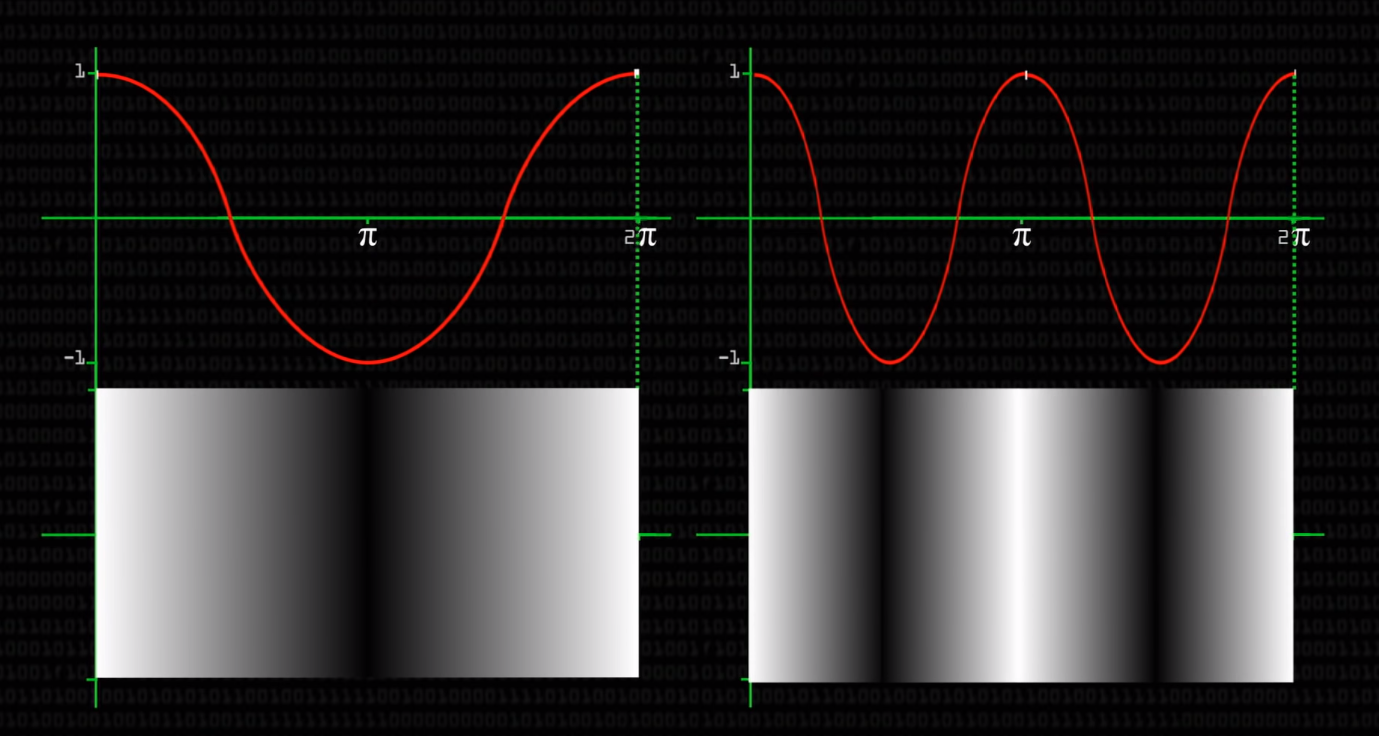
\includegraphics[scale=0.1]{figures/twocos.png}

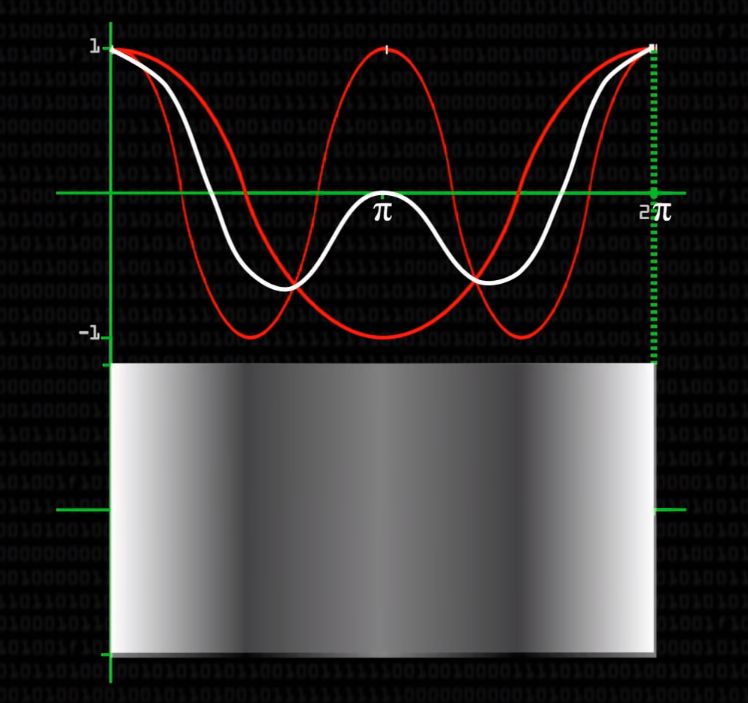
\includegraphics[scale=0.15]{figures/cossum.png}

\begin{footnotesize}
    forrás: JPEG DCT, Discrete Cosine Transform (JPEG Pt2)- Computerphile
\end{footnotesize}

\end{frame}

\subsection{Bázisfüggvények}
\begin{frame}{\secname : \subsecname}
\centering

\includegraphics[scale=0.3]{figures/Dctjpeg.png}

\begin{footnotesize}
    forrás: \url{en.wikipedia.org/wiki/JPEG}
\end{footnotesize}

\end{frame}

\subsection{Folyamat - 1: normalizálás} 
\begin{frame}{\secname : \subsecname}
\centering
Az értékből (0..255) kivonunk 128-at, így -128 és 127 közé kerülnek

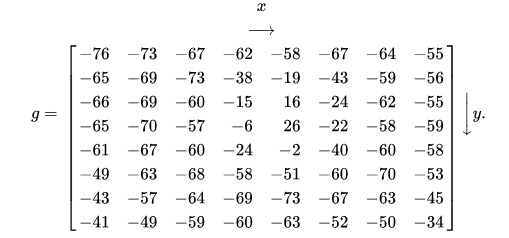
\includegraphics[scale=0.4]{figures/DCT_centered.png}
\end{frame}

\subsection{Folyamat - 2: Transzformáció}
\begin{frame}{\secname : \subsecname}
$ G_{u, v} = \frac{1}{4} \alpha(u) \alpha(v) \sum_{x=0}^{7}\sum_{y=0}^{7} g_{x, y} cos[\frac{(2x + 1) u \pi}{16}] cos[\frac{(2y + 1) v \pi}{16}]$


Transzformáció eredménye:

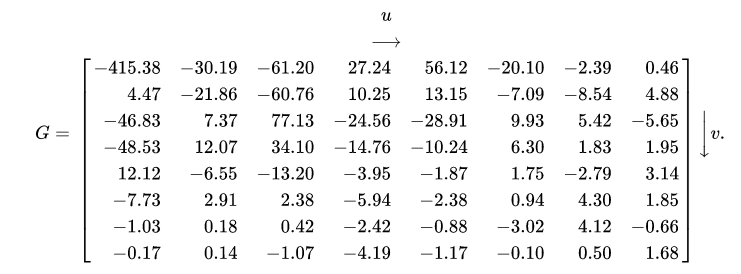
\includegraphics[scale=0.4]{figures/DCT_transformed.png}

\end{frame}

\subsection{Folyamat - 3: Kvantálás}
\begin{frame}{\secname : \subsecname}
\centering
Kvantálási mátrix 50 százalékos tömörítéshez

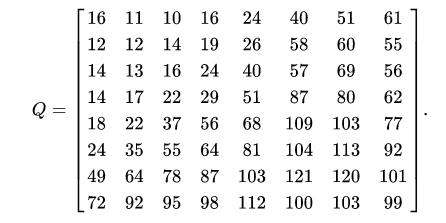
\includegraphics[scale=0.4]{figures/DCT_quant_50.png}

Végső együtthatók:

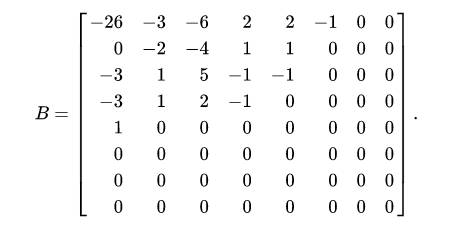
\includegraphics[scale=0.4]{figures/DCT_result.png}
\end{frame}


\begin{frame}
\centering
{\Huge Köszönöm a figyelmet!}
\end{frame}

\appendix{Források}
\begin{footnotesize}
    \begin{itemize}
        \item en.wikipedia.org/wiki/JPEG
        \item JPEG DCT, Discrete Cosine Transform (JPEG Pt1 \& Pt2)- Computerphile
        \item hu.wikipedia.org/wiki/Veszteségmentes\_tömörítés
        \item en.wikipedia.org/wiki/YCbCr
        \item www.journaldev.com/23246/huffman-coding-algorithm
        \item en.wikipedia.org/wiki/Chroma\_subsampling
        \item en.wikipedia.org/wiki/Discrete\_cosine\_transform
    \end{itemize}
\end{footnotesize}

\end{document}